\documentclass[a4paper,12pt]{article} 
\usepackage{mathrsfs}
\usepackage[utf8]{inputenc}
\usepackage[spanish]{babel}
\usepackage{amsmath}
\usepackage{amsfonts}
\usepackage{amssymb} 
\usepackage{graphicx} 
\usepackage{hyperref} 
\usepackage{wrapfig}
\usepackage{enumitem}
\usepackage{fancyhdr}
\usepackage{float}
\usepackage{eurosym}
\usepackage{color}
\usepackage{circuitikz}
\usepackage{titling}
\usepackage{hyperref}
\usepackage{media9}
\usepackage{lipsum}
\usepackage{tocbibind}
\usepackage{listings}
\usepackage{tabularx}
\usepackage{tcolorbox}
\usepackage{bookmark}
\usepackage{media9}
\usepackage[table]{xcolor}
\definecolor{lightblue}{RGB}{228, 244, 253}
\usepackage{listings}
\usepackage{color}

\definecolor{dkgreen}{rgb}{0,0.6,0}
\definecolor{gray}{rgb}{0.5,0.5,0.5}
\definecolor{mauve}{rgb}{0.58,0,0.82}

\lstset{frame=tb,
  language=Python,
  inputencoding=utf8,
  extendedchars=true,
  aboveskip=3mm,
  belowskip=3mm,
  showstringspaces=false,
  columns=flexible,
  basicstyle={\small\ttfamily},
  numbers=none,
  numberstyle=\tiny\color{gray},
  keywordstyle=\color{blue},
  commentstyle=\color{dkgreen},
  stringstyle=\color{mauve},
  breaklines=true,
  breakatwhitespace=true,
  tabsize=3,
  literate=%
    {á}{{\'a}}1
    {é}{{\'e}}1
    {í}{{\'i}}1
    {ó}{{\'o}}1
    {ú}{{\'u}}1
    {ñ}{{\~n}}1
    {č}{{\v{c}}}1
}
\usepackage[left=3cm,right=3cm,top=3cm,bottom=4cm]{geometry}
\sloppy

\pagestyle{fancy}
\providecommand{\abs}[1]{\lvert#1\rvert}
\providecommand{\norm}[1]{\lVert#1\rVert}

%%% Para las cabeceras
\newcommand{\hsp}{\hspace{20pt}}
\newcommand{\HRule}{\rule{\linewidth}{0.5mm}}
\headheight=50pt
%%% 
\newcommand{\vacio}{\textcolor{white}{ .}}

%%% Para que las ecuaciones se numeren
%%% con el número de sección y el de ecuación.
\renewcommand{\theequation}{\thesection.\arabic{equation}}


% Color azul para algunos 
% textos de la portada
\definecolor{azulportada}{rgb}{0.16, 0.32, 0.75}

%%%% Azul para textos de headings
\definecolor{azulinterior}{rgb}{0.0, 0.2, 0.6}

%%%%%%%%%%%%%%%%%%%%%%%%%%%%%%%%
%%%%%% Datos del proyecto %%%%%%
%%%%%%%%%%%%%%%%%%%%%%%%%%%%%%%%
%%%TÍTULO
%%% Escribirlo en minúsculas, el programa
%%% lo pondrá en mayúsculas en la portada.

\title{Extracción de características \\[1ex] y bolsa de palabras visuales}

%%%% AUTORES
\author{Lydia Ruiz Martínez \and Pablo Tuñón Laguna}

%%%%%%%%%%%%%%%%%%%%%
%%%%%%%%%%%%%%%%%%%%
\begin{document}

%%%%%%%%%%%%%%%%%%%%%%%%%%%%%%%
%%%%%%%%%%%%%%%%%%%%%%%%%%%%%%%
\begin{titlepage} %%%%% Aquí no hay que tocar nada.
	%%%% Las siguientes instrucciones generarán automáticamente
	%%%% la portada de tu proyecto.
	%%% Cambio de la estructura de esta página
\newgeometry{left=0.6cm,top=1.3cm,bottom=1.2cm}

\fbox{\parbox[c]{18.5cm}{
\begin{center}
\vspace{1.5cm}
{\fontfamily{ptm}\fontsize{24}{28.8}\selectfont{Universidad Pontificia de Comillas}}\\
[2.5em]
{\fontfamily{ptm}\fontsize{24}{5}\selectfont{ICAI}}\\
[3.5em]
{\fontfamily{ptm}\fontsize{28}{5}\selectfont{LABORATORIO 3}}\\
[2cm]
{\fontfamily{ptm}\fontsize{24}{5}\selectfont{Visión por Ordenador I}}\\
[2cm]

% Autor del trabajo de investigación
\textcolor{azulportada}{\fontfamily{ptm}\fontsize{16}{5}\selectfont{\theauthor}}\\
[2cm]
% Título del trabajo
\textcolor{azulportada}
{\fontfamily{ptm}\fontsize{30}{5}\selectfont{\textsc{\thetitle}}}\\
%{\Huge\textbf{\thetitle}}\\
[1.2cm]

\includegraphics[width=10cm]{data/Logo ICAI.png}
\\[1.8cm]

{\fontfamily{ptm}\fontsize{16}{5}\selectfont{Curso 2024-2025}}\\
[4cm]
\end{center}
}}
\end{titlepage}
 
 \restoregeometry
 %%%% Volvemos a la estructura de la página normal

%%%%%%%%%%%%%%%%%%%%%%%%%%%%%%

{%\Large

%%%Encabezamiento y pie de página
%%% También se genera automáticamente
%%% Mejor no tocarlo mucho.
\renewcommand{\headrulewidth}{0.5pt}
\fancyhead[R]{
\textcolor{azulportada}{\fontfamily{ptm}\fontsize{10}{3}\selectfont{Laboratorio 3 de Visión por Ordenador I}}\\
{\fontfamily{ptm}\fontsize{10}{3}\selectfont{\theauthor}}}
\fancyhead[L]{
  \textcolor{azulinterior}{\fontfamily{ptm}\fontsize{12}{4}\selectfont{\textbf{\thetitle}}}\\
}


\pagestyle{fancy}
\renewcommand{\footrulewidth}{0.5pt}
\fancyfoot[L]{\footnotesize Universidad Pontificia Comillas (ICAI) --- curso 2024-2025}
\fancyfoot[C]{\vacio}
\fancyfoot[R]{\footnotesize Página \thepage}

%%%%%%%%%%%%%%%%%%%%
\newpage

\renewcommand{\contentsname}{Índice}
\addtocontents{toc}{\protect\setcounter{tocdepth}{-1}} % Quita el índice de la tabla de contenidos
\tableofcontents
\addtocontents{toc}{\protect\setcounter{tocdepth}{2}}

\newpage


\newpage


\section{Introducción}


\vspace{1cm}

La visión por ordenador permite extraer y analizar características visuales a partir de imágenes digitales. El siguiente escrito se enfoca en la comprensión extracción de 
características así como en la construcción de una bolsa de palabras visuales, herramientas fundamentales para la clasificación de imágenes y la identificación de determinados patrones.

\vspace{0.5cm}

Se han estudiado múltiples técnicas de detección de características, estas pueden ser desde esquinas, líneas hasta diferentes puntos de interés. 
Para ello se han empleando métodos como los detectores de Harris y Shi-TOmasi en detección de esquinas, la transformada de Hough para líneas y detectores como 
\textit{SIFT} y \textit{KAZE} para la extracción de puntos de interés. Realizado el estudio de extracción, se han organizado dichas carcterísticas en una 
estructra de bolsa de palabras visuales. Esto permite la creación de un vocabulario el cual es útil para identisticas o tipos de imágenes nuevos con mayor rapidez.

\vspace{0.5cm}

El desarrolo del proyecto se ha realizado en Python mediante la librería OpenCV para la manipulación de imágenes y \textit{helpers} con métodos para obtener 
los resultados deseados. Con el fin de facilitar al lector que quiere consultar los resultados explicados en el escrito con el programa desarrollado, 
todo el procesado de imágenes se almacena en el fichero \textit{processed\_data} (el cual se crea automáticamente) teniendo este a su vez tres subcarpetas 
en la que se almacenan las imágenes, hay una para guardar la detección de esquinas (\textit{partA}), una para la de líneas (\textit{partB}) y finalmente una 
tercera para la detección de puntos de interés (\textit{partC}).

\newpage


\section{Detección de esquinas}


\vspace{1.cm}

A lo largo de la siguiente sección se va a explicar el desarrollo llevado a cabo para la detección de esquinas en imágenes digitales. Para ello se han empleado dos 
métodos diferentes, el detector de Harris y el detector de Shi-Tomasi. Ambos métodos se han aplicado a diferentes imágenes con el fin de comparar los resultados 
obtenidos. Sin embargo en un primer momento es necesario cargar las imágenes, para ello, se implementaron dos funciones de lectura que hacen uso de las librerías 
\textit{opencv} e \textit{imageio}. El método \textit{imread()} en opencv carga las imágenes en formato BGR, mientras que el mismo método en imageio carga las
imágenes en formato RGB. Esto produce una alteración en la organización de los colores de la imagen a tener en cuenta ya que algunos métodos de detección de esquinas
pueden ser sensibles a los colores.

\vspace{0.5cm}

\begin{figure}[h!]
    \centering
    \begin{minipage}[b]{0.45\textwidth}
        \centering
        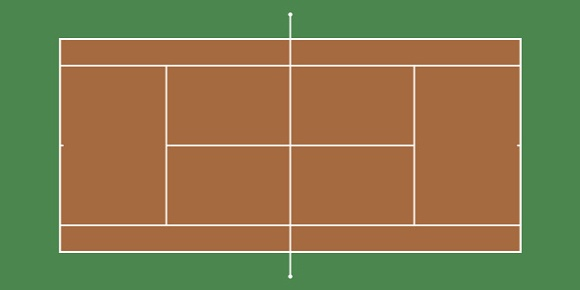
\includegraphics[width=\textwidth]{data/processed_data/partA/imageio_blue_tennis_court.jpg}
        \caption{Carga de pista de tenis a través de \textit{imageio} (RGB), autoría propia.}
        \label{fig:tennis-imageio}
    \end{minipage}
    \hfill
    \begin{minipage}[b]{0.45\textwidth}
        \centering
        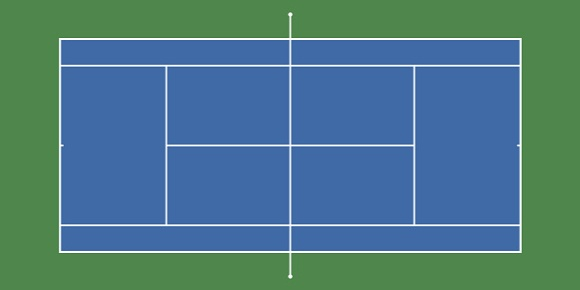
\includegraphics[width=\textwidth]{data/processed_data/partA/opencv_blue_tennis_court.jpg}
        \caption{Carga de pista de tenis a través de \textit{opencv} (BGR), autoría propia.}
        \label{fig:tennis-opencv}
    \end{minipage}

\end{figure}

\vspace{0.5cm}

La detección de esquinas se realiza localizando en la imagen procesada cambios fuertes en el gradiente de la imágen, es decir, cambios en la intensidad de los píxeles.
Es por ello que tanto para el método de Harris como para el de Shi-Tomasi se ha convertido la imagen a escala de grises. Para ello se ha utilizado el método \textit{cv2.cvtColor()}
(cargándola previamente con el método de \textit{opencv}).

\newpage


\subsection{Método de Harris}

\vspace{0.5cm}

El método de Harris estudia la variación de la intensidad comentada como una comparación de la intensidad de los píxeles vecinos en todas las direcciones, sumando 
posteriormente los cuadrados de las diferencias:

\vspace{0.5cm}

\begin{equation}
    E(u,v) = \sum_{x,y \ \in W} [I(x+u, y+v) - I(x,y)]^2
\end{equation}

\vspace{0.5cm}

Dicha pequeña variación de los píxeles cercanos evaluados se puede entender como una derivada discreta, por lo que realizando una aproximación de Taylor de primer orden
se puede obtener lo siguiente:

\vspace{0.5cm}

\[
\begin{aligned}
    E(u,v) &\approx \sum_{x,y \ \in W} [I_xu - I_yv]^2 = \sum_{x,y \ \in W}(u^2I_x^2 + 2uvI_xI_y + v^2I_y^2) \\
    A &= \sum_{x,y \ \in W} I_x^2; \quad B = \sum_{x,y \ \in W} I_xI_y; \quad C = \sum_{x,y \ \in W} I_y^2 \\
\end{aligned}
\]

\vspace{0.5cm}

Por todo lo anterior se puede obtener la matriz de Harris, presente en la expresión:

\vspace{0.5cm}

\begin{equation}
    E(u, v) \approx [u \ v] \begin{bmatrix} A & B \\ B & C \end{bmatrix} \begin{bmatrix} u \\ v \end{bmatrix}
\end{equation}

\vspace{0.5cm}

A partir de los distintos valores de la matriz de Harris se puede saber si el conjunto de píxeles evaluados corresponden a una esquina, un borde o una región plana:

\vspace{0.5cm}

\begin{itemize}
    \item Si A = B = C = 0, entonces se trata de una región plana (no hay variación en ninguna dirección.
    \item Si A = B = 0 y C != 0, entonces se trata de un borde horizontal.
    \item Si A != 0 y B = C = 0, entonces se trata de un borde vertical.
    \item Si A != 0, B != 0 y C!= 0 , entonces se trata de una esquina (cambio significativo en todas las direcciones).
\end{itemize}

\vspace{0.5cm}

Explicado el fundamento matemático, la parte programística se ha llevado a cabo mediante la función \textit{cv2.cornerHarris()}
que recibe como parámetros la imagen en escala grises, el tamaño de píxeles a evaluar alrededor del píxel central, 
el tamaño de la apertura del kernel de Sobel (ya que se utiliza para calcular los gradientes) y el valor de la constante de Harris, que 
en la función permite afinar la sensibilidad del detector. A continuación se muestra la extracción de esquinas mediante el método explicado:

\vspace{0.5cm}

\begin{figure}[h!]
    \centering
    \begin{minipage}[b]{0.35\textwidth}
        \centering
        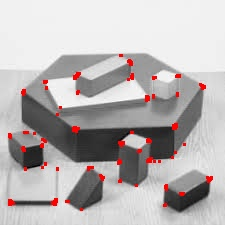
\includegraphics[width=\textwidth]{data/processed_data/partA/harris_geometry.jpg}
        \caption{Extracción de esquinas mediante el método de Harris para geometry, autoría propia.}
        \label{fig:harris-geometry}
    \end{minipage}
    \hfill
    \begin{minipage}[b]{0.45\textwidth}
        \centering
        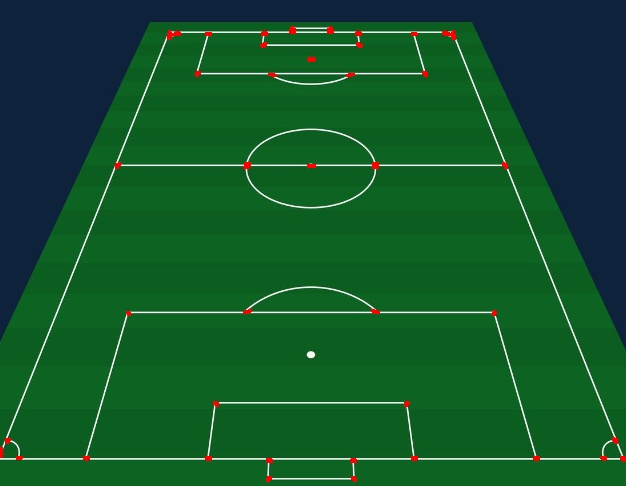
\includegraphics[width=\textwidth]{data/processed_data/partA/harris_football.jpg}
        \caption{Extracción de esquinas mediante el método de Harris para football, autoría propia.}
        \label{fig:harris-football}
    \end{minipage}

\end{figure}

\vspace{0.5cm}

\begin{figure}[h!]
    \centering
    \begin{minipage}[b]{0.4\textwidth}
        \centering
        \includegraphics[width=\textwidth]{data/processed_data/partA/harris_sudoku.jpg}
        \caption{Extracción de esquinas mediante el método de Harris para sudoku, autoría propia.}
        \label{fig:harris-sudoku}
    \end{minipage}
    \hfill
    \begin{minipage}[b]{0.45\textwidth}
        \centering
        \includegraphics[width=\textwidth]{data/processed_data/partA/harris_tennis.jpg}
        \caption{Extracción de esquinas mediante el método de Harris para tennis, autoría propia.}
        \label{fig:harris-tennis}
    \end{minipage}

\end{figure}

\newpage

\subsection{Método de Shi-Tomasi}

El método de Shi-Tomasi presenta algunas mejoras sobre el método de Harris. Este método selecciona las esquinas en 
función del valor mínimo de los autovalores de la matriz de Harris, resultando en una detección de esquinas más robusta en 
condiciones variables de iluminación y textura:

\vspace{0.5cm}  

\begin{itemize}
    \item Si \( \lambda_1 \approx 0 \) y \( \lambda_2 \approx 0 \), entonces se trata de una región plana (no hay variación significativa en ninguna dirección).
    \item Si \( \lambda_1 \gg 0 \) y \( \lambda_2 \approx 0 \), entonces se trata de un borde horizontal (o veritcal si se intercambia la relación de los autovalores).
    \item Si \( \lambda_1 \gg 0 \) y \( \lambda_2 \gg 0 \), entonces se trata de una esquina (variación en ambas direcciones).
\end{itemize}

\vspace{0.5cm}

La función \textit{cv2.goodFeaturesToTrack()} permite la detección de esquinas mediante el método de Shi-Tomasi. Esta función recibe como parámetros la imagen en escala de grises,
el número de esquinas a detectar, la calidad mínima de la esquina (valor entre 0 y 1) y la distancia mínima entre las esquinas detectadas. A continuación se muestra la extracción 
de esquinas mediante el método de Shi-Tomasi realizando un una circunferencia de 4 píxeles en torno a ellos en distintos colores:

\vspace{0.5cm}

\begin{figure}[h!]
    \centering
    \begin{minipage}[b]{0.35\textwidth}
        \centering
        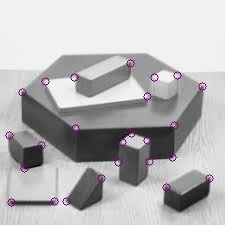
\includegraphics[width=\textwidth]{data/processed_data/partA/shi_tomasi_geometry.jpg}
        \caption{Extracción de esquinas mediante el método de Shi-Tomasi para sudoku, autoría propia.}
        \label{fig:shi-tomasi-geometry}
    \end{minipage}
    \hfill
    \begin{minipage}[b]{0.45\textwidth}
        \centering
        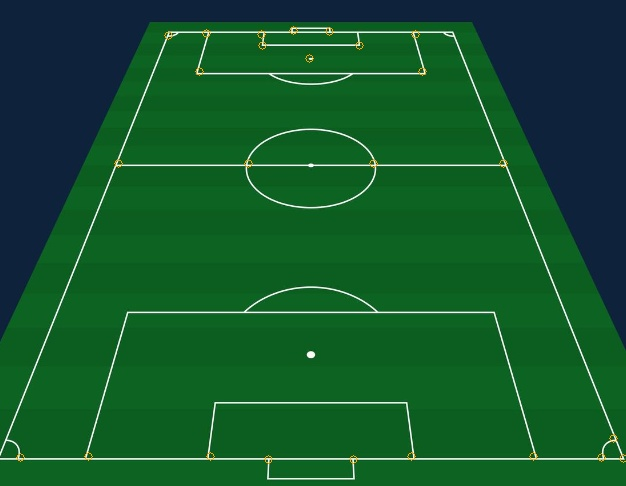
\includegraphics[width=\textwidth]{data/processed_data/partA/shi_tomasi_football.jpg}
        \caption{Extracción de esquinas mediante el método de Shi-Tomasi para football, autoría propia.}
        \label{fig:shi-tomasi-football}
    \end{minipage}

\end{figure}

\newpage

\begin{figure}[h!]
    \centering
    \begin{minipage}[b]{0.35\textwidth}
        \centering
        \includegraphics[width=\textwidth]{data/processed_data/partA/shi_tomasi_sudoku.jpg}
        \caption{Extracción de esquinas mediante el método de Shi-Tomasi para sudoku, autoría propia.}
        \label{fig:shi-tomasi-sudoku}
    \end{minipage}
    \hfill
    \begin{minipage}[b]{0.45\textwidth}
        \centering
        \includegraphics[width=\textwidth]{data/processed_data/partA/shi_tomasi_tennis.jpg}
        \caption{Extracción de esquinas mediante el método de Shi-Tomasi para tennis, autoría propia.}
        \label{fig:shi-tomasi-tennis}
    \end{minipage}

\end{figure}

\newpage


\section{Detección de líneas}


\vspace{1cm}

La detección de líneas permite la identificación de los segmentos que unen los bordes anteriormente detectados en la sección anterior.
A lo largo de la siguiente sección se va a exponer el funcionamiento de la transformación de Hough como extractor de líneas. 
El fundamento matemático de la detección de líneas se basa en la ecuación de la recta en forma explícita:

\vspace{0.5cm}

\begin{equation}
    y = mx + n
\end{equation}

\vspace{0.5cm}

Se recorre cada conjunto de puntos de la imagen donde se han detectado bordes y se calcula la ecuación de la recta que los une. En el plano (x,y)
hay infinitas rectas que pasan por un punto dado, sin embargo, en el espacio de parámetros (m,n) hay una única recta que pasa por dicho punto. Sería
como invertir los parámetros de la recta, donde en lugar de tratar de obtener y a partir de x, se trata de obtener n a partir de m.

\vspace{0.5cm}

La transformación anterior es útil de la siguiente manera, una vez se tiene una recta en el plano (m,n) se calcula la recta del posterior punto
perteneciente al borde en el plano (m,n). La recta que une los dos puntos del plano (x,y) (que no son más que puntos de un borde detectado) es 
el punto de intersección de las rectas en el plano (m,n). Una vez que se encuentra dicha recta se disponen en una máscara de ceros (del mismo tamaño
que la imagen evaluada) unos que permiten identificar la recta, dicha máscara se actualiza con cada recta encontrada.

\vspace{0.5cm}

Sin embargo el método anteriormente explicado falla en la identificación de líneas verticales, debido a que la pendiente de la recta es infinita.
Es por ello que se hace un razonamiento análogo pero en lugar de usar coordenadas cartesianas se usan coordenadas polares, donde la recta se define
como:

\vspace{0.5cm}

\begin{equation}
    \rho = x \cos(\theta) + y \sin(\theta)
\end{equation}

\vspace{0.5cm}

En este nuevo caso el espacio al que se realiza la transformada es el plano (\(\rho, \theta\)), donde en lugar de tratar con intersección de rectas se
realiza con intersección de sinusoidales.

\vspace{0.5cm}

Programísticamente el porcedimiento es similar aunque ciertas funciones de \textit{opencv} permiten la abstracción de la transformación y la intersección iterativa.
Se comienza detectando los bordes de la imagen en blanco y negro a través de la función \textit{Canny} que destaca los contornos de los objetos presentes en la imagen. 
La función usada requiere de un ajuste en los parámetros low\_threshold y high\_threshold, los cuales controlan la sensibilidad a los bordes y permiten 
reducir el ruido en la imagen. La función devuelve una imagen binaria, donde los píxeles que forman los bordes tienen valor blanco (255) y el fondo es negro (0).
A continuación se puede observar la extracción de bordes realizada con Canny:

\vspace{0.5cm}

\begin{figure}[h!]
    \centering
    \begin{minipage}[b]{0.35\textwidth}
        \centering
        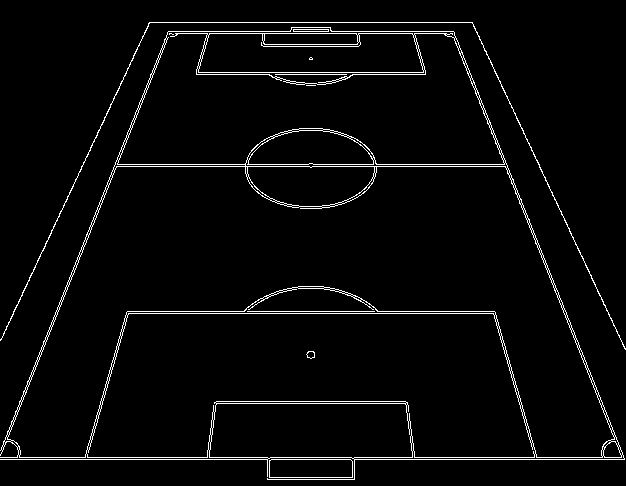
\includegraphics[width=\textwidth]{data/processed_data/partB/canny_football.jpg}
        \caption{Extracción de bordes de football mediante Canny, autoría propia.}
        \label{fig:canny-football}
    \end{minipage}
    \hfill
    \begin{minipage}[b]{0.45\textwidth}
        \centering
        \includegraphics[width=\textwidth]{data/processed_data/partB/canny_sudoku.jpg}
        \caption{Extracción de bordes de sudoku mediante Canny, autoría propia.}
        \label{fig:canny-sudoku}
    \end{minipage}

\end{figure}

\vspace{0.5cm}

Para identificar líneas en la imagen a partir de los bordes obtenidos, se utiliza la transformada de Hough mediante \textit{HoughLinesP}, que detectará
las líneas a partir de los bordes identificados. La función recibe los bordes, $\rho$ que es un parámetro que permite identificar sinusoidales desde 0 hasta dicho valor (en este caso 
$\pi/180$), la longitud mínima de la línea y la máxima entre líneas así como un threshold. Este threshold permite que sólo se identifiquen las líneas que sean n veces coincidentes
con el fin de reducir el posible ruido en la imagen. El resultado de la función es una lista que contiene los puntos iniciales y finales de cada recta detectada. 

\vspace{0.5cm}

Tras obtener las líneas presentes en la imagen, se usa la función \textit{line} que dibuja una recta dado una coordenada de inicio y de final así como 
un grosor y color para la recta. Cabe destacar que el proceso explicado anteriormente puede extraer tanto líneas rectas como curvas. Esto se comnsigue 
mediante el afinando del parámetro de mínima longitude de líneas así como el de máxima distancia entre ellas. Esto se debe al hecho de que dos píxeles 
alineados en una imagen forman una recta y dado que las imágenes a procesar están compuestas de píxeles y no de vectores (de momento imposibles en una 
imagen digital) son posibles de obtener.

\newpage

\begin{figure}[h!]
    \centering
    \begin{minipage}[b]{0.35\textwidth}
        \centering
        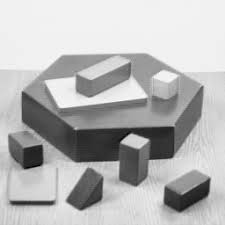
\includegraphics[width=\textwidth]{data/processed_data/partB/hough_geometry.jpg}
        \caption{Extracción de líneas de geometry mediante Hough, autoría propia.}
        \label{fig:hough-geometry}
    \end{minipage}
    \hfill
    \begin{minipage}[b]{0.45\textwidth}
        \centering
        \includegraphics[width=\textwidth]{data/processed_data/partB/hough_football.jpg}
        \caption{Extracción de líneas de football mediante Hough, autoría propia.}
        \label{fig:hough-football}
    \end{minipage}

\end{figure}


\begin{figure}[h!]
    \centering
    \begin{minipage}[b]{0.3\textwidth}
        \centering
        \includegraphics[width=\textwidth]{data/processed_data/partB/hough_sudoku.jpg}
        \caption{Extracción de líneas de sudoku mediante Hough, autoría propia.}
        \label{fig:hough-sudoku}
    \end{minipage}
    \hfill
    \begin{minipage}[b]{0.5\textwidth}
        \centering
        \includegraphics[width=\textwidth]{data/processed_data/partB/hough_tennis.jpg}
        \caption{Extracción de líneas de tennis mediante Hough, autoría propia.}
        \label{fig:hough-tennis}
    \end{minipage}

\end{figure}

\newpage


\section{Estudio de puntos de interés}


\vspace{1cm}

Un punto de interés es un píxel o conjunto de píxeles que destacan por su singularidad en la imagen. Estos puntos son útiles para la identificación de objetos
en una imagen, ya que permiten la comparación de características entre distintas imágenes. A lo largo de la siguiente sección se va a explicar la 
extracción algo más manual de los puntos. Posteriormente se emplarán funciones de opencv para la extracción de puntos de interés de forma más eficiente y automática,
con dichos puntos de interés se construirá una bolsa de palabras y se mostrará la eficiencia en la clasificación de la misma.

\vspace{0.5cm}

\subsection{Extracción manual de puntos de interés} 

\vspace{0.5cm}

Para la extracción de puntos de interés se ha empleado la imagen geometry mientras que para una posterior verificación se ha usado una rotación de 90º horarios de la misma.
El proceso a replicar es el realizado por \textit{SIFT} (Scale-Invariant Feature Transform), este comienza aplicando varios filtros gaussianos de distintas $\sigma$ a la imagen.
La utilidad de aplicar dichas máscaras es la de obtener distintas escalas de la imagen, ya que un punto de interés puede ser detectado en una escala y no en otra. Es decir, aplicando
dichas máscaras se obtiene una imagen con distintos niveles de emborronado, el objetivo es que de cada uno de los niveles se pueda extraer una serie de puntos de interés. Esto es
posible debido a la naturaleza del filtro gaussiano, que al difuminar las zonas, resalta los bordes relevantes (cambios de intensidad) de la imagen.

\vspace{0.5cm}

Las distintas escalas de emborronado se obtienen a través de \textit{generateGaussianSigmas}, que recibe la $\sigma$ inicial y el número de escalas a obtener, devolviendo una lista
con las distintas $\sigma$ a aplicar. Posteriormente se toma cada una de esos valores y se aplica un filtro gaussiano a la imagen original (que fue cargada y convertida a escala de grises)
mediante la función \textit{GaussianBlur}, dicha función requiere de una imagen y una $\sigma$ para aplicar el filtro. Cabe destacar que se aplica una y otra vez la función sobre la imagen
ya emborronada almacenándola en distintos estados, esto se hace para que las máscaras tengan un efecto de difuminado acumulativo.

\vspace{0.5cm}

Una vez que se poseen dichas imágenes, se diferencia cada imagen con la posterior, de esta manera, únicamente los puntos que permanecen después del emborronado quedan presentes en la imagen.
Dichos puntos se almacenan en imágenes binarias, estas son producidas por la función \textit{substract} the opencv. Dicha función requiere de las dos escalas, la actual y la posterior.

\vspace{0.5cm}

El siguiente paso consiste en la identificación de máximos o mínimos locales en la imagen binaria, con este objetivo se ha desarrollado una función \textit{isPixelAnExtremum}. Dicha función
toma 3 cuadrículas de 3x3 píxeles, identifica el píxel central de la segunda cuadrícula y verifica que en valor absoluto es mayor a un threshold (proporcionado por el llamado de la función)
y evalúa que dicho punto sea mayor, menor o igual a todos y cada uno de los píxeles de la cuadrícula central y las adyacentes. Si cumple con dichas condiciones se considera un punto de interés,
ya que aquellos puntos que permanecen a lo largo de todas las escalas o que nunca aparecen (por efecto del emborronado) son puntos de interés.

\vspace{0.5cm}

Se deja el siguiente ejercicio de imaginación al lector:

\vspace{0.5cm}

\begin{itemize}
    \item Imagine una toroide en un espacio tridimensional con un agujero no demasiado grande. Dicho agujero además es el origen de coordenadas.
    \item Ahora imagine que el toroide se emborrona gradualmente. Las fronteras se difuminan cada vez más, los bordes no son precisos, sin embargo puede seguir identificando el toroide. Tal vez ya no percibe su profundidad, pero es capaz de ver parcialmente su sombra y desde luego ve el agujero del centro.
    \item Al diferenciar las imágener emborronadas, los puntos que permanecen son los que definen el toroide, los que no, son los que se han difuminado.
    \item El origen de coordenadas o centro del toroide, al no haber variado nunca, está presente en todas las imágenes. Es por ello que cuando traza una cuadrícula de 3x3 píxeles alrededor de dicho punto y lo compara con el resto de imágenes diferenciadas, siempre será un máximo o un mínimo (según el emborronado y el color original).
\end{itemize}

\vspace{0.5cm}

Se espera que con el ejercicio anterior se haya podido comprender algo mejor el proceso de extracción enunciado con anterioridad. Se ha enunciado el proceso para extraer el punto de interés a partir
de un conjunto de cuadrículas de 9 píxeles, sin embargo las imágenes tienen un tamaño considerablemente mayor. Para procesar los puntos de interés de la imagen se ha desarrollado la función \textit{findScaleSpaceExtrema}.
Esta función necesita las imágenes difuminadas, las imágenes diferenciadas, los distintos $\sigma$ y un threshold para la identificación de los puntos de interés. La función recorre cada píxel del interior de la imagen
(no toma los píxeles de los bordes para poder realizar la verificación de máximos y mínimos locales) y evalúa si dicho píxel es un punto de interés. En caso de serlo, se ajusta la localización del punto de interés
en la imagen original con un ajuste cuadrático, se obtiene la orientación y finalmente se almacena para su posterior uso.

\vspace{0.5cm}

Finalmente se crean descriptores para cada punto de interés, estos son vectores que describen la orientación, localización y distribución de los píxeles alrededor del punto de interés. Dichos descriptores 
son útiles para la comparación e identificación de puntos de interés y se obtienen a través de la función \textit{generateDescriptors} a partir de los puntos de interés y de las escalas de emborronado.

\vspace{0.5cm}

Cabe destacar que todos los procesos y funciones anteriormente descritos fueron unidos en la función \textit{computeKeypointsAndDescriptors} que sólo necesita la imagen original, el primer $\sigma$ y el número de intervalos
y devuelve los puntos de interés y sus descriptores. Para ejemplificar se usa la función \textit{matchFeatures} que al recibir los descriptores de dos imágenes, compara los puntos de interés y devuelve una imagen con la unión de 
los mismos:

\vspace{0.5cm}

\begin{figure}[h!]
    \centering
    \begin{minipage}[b]{0.4\textwidth}
        \centering
        \includegraphics[width=\textwidth]{data/processed_data/partC/matches.jpg}
        \caption{Verificación de puntos de interés y orientación manual, autoría propia.}
        \label{fig:keypoints-detection}
    \end{minipage}
    \hfill
    \begin{minipage}[b]{0.4\textwidth}
        \centering
        \includegraphics[width=\textwidth]{data/processed_data/partC/matches_opencv.jpg}
        \caption{Verificación de puntos de interés y orientación con opencv, autoría propia.}
        \label{fig:keypoints-detection-opencv}
    \end{minipage}
\end{figure}

\vspace{0.5cm}

Tal y como se puede observar (y como cabía esperar), la extracción manual de puntos de interés, aunque correcta, es un proceso lento y menos eficiente que el realizado por la implementación de \textit{opencv} 
(la cual se explicará en la próxima sección). Se prefiere la implementación no manual no sólo por la eficiencia sino por la robustez y precisión de la misma obteniendo un mayor número de puntos de interés y descriptores.

\vspace{0.5cm}

\subsection{Trabajo con bolsas de palabras visuales}

\vspace{0.5cm}

Tal y como se ha enunciado a lo largo del escrito, una bolsa de palabras es un conjunto de puntos de descriptores que permiten la clasificación de imágenes y objetos a partir de comparaciones de características propias de cada imagen.
Dado que en la anterior sección se identificó la eficiencia de la extracción de puntos de interés con \textit{opencv} por encima de la extracción manual, se va a analizar dicha implementación para usarla en la creación de una bolsa de palabras.

\vspace{0.5cm}

El proceso comienza creando un extractor de descriptores, en la sección anterior se usó \textit{$SIFT_create$} que generará un extractor que sigue el algoritmo \textit{SIFT} pero se pueden crear otros descriptores que se ajusten a las necesidades del problema.
Posteriormente se extraen los descriptores y puntos de interés de una imagen en escala de grises mediante el método \textit{detectAndCompute} del extractor. 

\vspace{0.5cm}

Explicado ya el proceso de extracción de \textit{opencv} se ha desarrollado un fichero Python: \textit{words\_bag.py} que permite la creación de una bolsa de palabras visuales así como la clasificación de distintas imágenes todo ello con 
distintos parámetros y descriptores. Las pruebas se han realizado sobre las imagenes de un dataset con 2981 imágenes de entrenamiento y 1501 de test y se han recogido las 32 ejecuciones en el fichero anexo \textit{results.csv}.

\vspace{0.5cm}

\subsubsection{Creación de la bolsa de palabras visuales}
Los pasos para la creación de la bolsa de palabras visuales son los siguientes:

\vspace{0.5cm}

\begin{itemize}
    \item Creación del extractor de descriptores ya sea con \textit{$SIFT_create$} o con \textit{$KAZE_create$} (se quisieron evaluar más extractores pero los programas proporcionados de validación no estaban adaptados, cosa que se hará de cara al desarrollo del \"AirTrackPad\")
    \item Extracción de los descriptores y puntos de interés de las imágenes en escala de grises de entrenamiento con el método \textit{detectAndCompute} del extractor.
    \item Creación de un vocabulario con un tamaño determinado de vocabulario y un número de iteraciones, ya que se realiza un clustering a través de K-Means de los descriptores para obtener las palabras visuales.
    \item Guardado del vocabulario en un fichero \textit{$descriptor_parameters_vocabulary.pickle$} para su posterior uso.
    \item Cargado del vocabulario para el entrenamiento de un clasificador a través de la clase \textit{Bow} y el método \textit{$load_vocabulary$}.
    \item Entrenamiento de un clasificador de imágenes de la clase \textit{ImageClassifier} con el vocabulario cargado y el método \textit{train} (que recibe el training set). Este proceso devuelve el clasificador entrenado, este es guardado en una combinación del fichero \textit{$descriptor_parameters_labels.json$} y el fichero \textit{$descriptor_parameters_model.xml$} para su posterior uso.
    \item Inferencia en el conjunto de entrenamiento con el método \textit{predict} del clasificador entrenado. Este método devuelve las etiquetas inferidas y la precisión de la clasificación.
    \item Inferencua en el conjunto de test con el método \textit{predict} del clasificador entrenado. Este método devuelve las etiquetas inferidas y la precisión de la clasificación.
\end{itemize}

\vspace{0.5cm}

\subsubsection{Muestreo de resultados}

Se ha realizado un total de 32 pruebas con las siguientes modificaciones:

\vspace{0.5cm}

\begin{itemize}
    \item Se ha variado el tamaño del vocabulario entre: 50, 100, 200 y 400.
    \item Se ha variado el número de iteraciones entre: 10, 20, 30 y 40.
    \item Se ha variado el extractor de descriptores entre \textit{SIFT} y \textit{KAZE}, cabe destacar que \textit{SURF} y \textit{AKAZE} (las versiones rápidas y optimizadas de los anteriores) no se pudieron probar debido a que fueron publicados y por tanto limitados al uso público. Del mismo modo queda pendiente adaptar los programas de entrenamiento y validación para probar \textit{FAST}, \textit{ORB} y \textit{BRISK}.
\end{itemize}

\vspace{0.5cm}

Después de unas 15h de ejecución, se obtuvieron resultados concluyentes respecto a los parámetros a usar así como el extractor de descriptores óptimo:

\vspace{0.5cm}

\begin{itemize}
    \item El extractor de puntos de interés \textit{KAZE} es considerablemente más lento e ineficiente que \textit{SURF} consiguiendo siempre menor precisión para los mismos parámetros, así mismo es más ineficiente temporalmente. Prácticamente en todo momento hay una diferencia de 0.09 en la precisión de la clasificación, en test y en train.
    \item El número de iteraciones óptimo en ambos extractores está entre 20 y 30, siendo 30 algo más común, sería interesante realizar ciertas pruebas con 25 y 35 iteraciones para ver si se obtiene una mejora en la precisión.
    \item Aparentemente cuanto mayor es el número de palabras en el vocabulario, mayor es la precisión en la clasificación, aumentar dicho valor aumenta casi exponencialmente el tiempo de creación de vocabulario. A pesar de ello, el tiempo de evaluación y entrenamiento aumenta de forma lineal (aparentemente) por lo que dado que el vocabulario sólo se genera una vez y se almacena, sería interesante aumentar todavía más el número de palabras en el vocabulario y observar si hay un aumento en la eficiencia de la clasificación, ya que el máximo valor se ha obtenido con 400 palabras en el vocabulario.
\end{itemize}

Por todo lo anterior se ha decidido que la mejor combinación de parámetros y extraxctores (a falta de realizar más pruebas es la siguiente):

\vspace{0.5cm}

\begin{itemize}
    \item Tamaño del vocabulario: 400
    \item Número de iteraciones: 20
    \item Extractor de descriptores: \textit{SIFT}
    \item Accuracy en train: 0.811
    \item Accuracy en test: 0.521
    \item Tiempo de ejecución de aproximado: 18 minutos
\end{itemize}

\vspace{0.5cm}

La mejor versión de \textit{KAZE} ha sido:

\vspace{0.5cm}

\begin{itemize}
    \item Tamaño del vocabulario: 400
    \item Número de iteraciones: 20
    \item Extractor de descriptores: \textit{KAZE}
    \item Accuracy en train: 0.685
    \item Accuracy en test: 0.437
    \item Tiempo de ejecución de aproximado: 29 minutos
\end{itemize}

\vspace{0.5cm}

Del mismo modo se recomienda para futuras pruebas aumentar el conjunto de entrenamiento para tener una mayor precisión en el entrenamiento (tratando siempre de no realizar overfitting), realizar pruebas con otros extractores de descriptores, probar 25 y 35 iteraciones y aumentar el tamaño del vocabulario a 500 y 600 palabras para observar si hay una mejora en la precisión de la clasificación.
\end{document}



